\documentclass{article}%Explained in due time
%Math Stuff
\usepackage{amsmath} % many display options for math modes and such (VERY IMPORTANT)
\usepackage{physics} % useful math symbols and macros (VERY IMPORTANT)
\usepackage{amssymb} % heck ton of math symbols and fonts (VERY IMPORTANT)
\usepackage{amsfonts} % Additional fonts, math symbols, and options for existing fonts (IMPORTANT)
\usepackage{mathtools} % lots of cool mathtools oh wait that is the name (IMPORTANT)
\usepackage{siunitx} % allows you to quickly define units within math mode (IMPORTANT)
\usepackage{array} % allows you to write piece-wise functions, matrices, and other cool things (IMPORTANT)
\usepackage{txfonts} % defines times new roman as default text font and provides supporting math symbols
\usepackage{braket} % allows the use of detailed Dirac braket notation
\usepackage{cancel} % used to cancel terms (with X or diagonal line) while writing math (useful for assignments)
\usepackage{ulem} % underlines, typewriter font (for comp sci somewhat), and striking out (required for cancel package)
%\usepackage{halloweenmath} % spooky
\usepackage{empheq} %Extension of amsmath for boxing equations or answers


%Formatting Stuff
\usepackage[utf8]{inputenc} % the typesetting rules
\usepackage[left = 22mm, right = 22mm]{geometry} % flexible and easy interface to change page dimensions
\usepackage{graphicx} % provides additional options for figures
\usepackage{float} % allows you to tell latex no really I want the figure HERE (with H)
\usepackage{color} % provides coloring capabilities to everything
\usepackage{fancyhdr} % making fancy headers (obviously)
\usepackage{changepage} % allows to change page formatting in the middle of a document (rather than the same throughout) 
\usepackage{enumitem} % better control over enumerate and itemize
\usepackage[labelfont=bf]{caption} % altering options for captions
\usepackage{sidecap} % allows sideways captions for figures and tables
\usepackage{soul,xcolor} % can enhance striking, underlining, and highlighting (in non-math mode)


%Stuff for Tables
\usepackage{booktabs} % allows weird lines within tables
\usepackage{multirow}
\usepackage{multicol} % allows for multiple columns and rows that collapse into single columns
\usepackage{longtable} % allows a table to run over multiple pages
\usepackage{colortbl} % colourful tables!

%Stuff for Citing
%\usepackage{apacite} % helps you apa cite
%\usepackage[numbers]{natbib} % implements both author-year and numbered references
\usepackage{url} % allows options for url links
\usepackage[colorlinks, citecolor = black, urlcolor = black, linkcolor = black]{hyperref} %references (citation) options and hyperlink integration


%Chemistry Stuff
\usepackage[version=4]{mhchem} % write chemical equations within math mode
\usepackage{chemfig} % draw simple and complex chemical structures in latex

%Elijah Adams Created Commands
\newcommand{\Q}{\mathbb{Q}} %Mathematical sets
\newcommand{\R}{\mathbb{R}}
\newcommand{\C}{\mathbb{C}}
\newcommand{\Z}{\mathbb{Z}} 
\newcommand{\Curl}{\vec{\nabla}\times} % Good looking curl and div and laplace (because physics package ones look like shit)
\newcommand{\Div}{\vec{\nabla}\cdot}
\newcommand{\laplace}{\vec{\nabla}^2}
\newcommand{\yas}{\frac{1}{4\pi\epsilon_0}} % Useful for E&M stuff
\newcommand{\mas}{\frac{\mu_0}{4\pi}}
\newcommand{\ppdv}[2]{\frac{\partial^2 #1}{\partial #2^2}} % Twice partial derivatives

\setlength{\parindent}{4mm}
\definecolor{purple}{rgb}{0.84,0.71,0.85} % defining a colour for later, each rgb value is a ratio of r/255, g/255 and b/255 because 255 is the maximum value of rgb numbers
\newcolumntype{d}{>{\columncolor{purple}}c} 

%explained in due time


\begin{document}

%Lab report notes: Make sure to convey your thought process (Very important!). Detail your process, document what you're doing while you're doing it. Be clear as to why you're doing a certain an analysis, why you're using this equation, why do you have an uncertainty of this type, why are you using this uncertainty propagation method. 

%Citations: Site the lab manual and the uncertainty manual.

\begin{titlepage} % Suppresses headers and footers on the title page
	\centering % Centre everything on the title page
	\scshape % Use small caps for all text on the title page
	\vspace*{\baselineskip} % White space at the top of the page
	\rule{\textwidth}{1.6pt}\vspace*{-\baselineskip}\vspace*{2pt} % Thick horizontal rule
	\rule{\textwidth}{0.4pt} % Thin horizontal rule

	\vspace{0.75\baselineskip} % Whitespace above the title
	
	{\LARGE TEMPLATE \LaTeX\:Lab Report 2025\\(Replace with name of experiment)} % Title
	
	\vspace{0.75\baselineskip} % Whitespace below the title
	
	\rule{\textwidth}{0.4pt}\vspace*{-\baselineskip}\vspace{3.2pt} % Thin horizontal rule
	\rule{\textwidth}{1.6pt} % Thick horizontal rule
	
	\vspace{2\baselineskip} % Whitespace after the title block
	Physics 36X Laboratory \#\# \\ % Subtitle or further description
	\vspace*{3\baselineskip} % Whitespace under the subtitle
	DATE \today \\ TA: \\ Group number:
	\vspace{5.0\baselineskip} % Whitespace before the editors

	{\scshape\Large Names of everyone in the lab group
 
One person per line
\\ } % Editor list
	\vspace{1.0\baselineskip} % Whitespace below the editor list
	\textit{The University of Calgary} % Editor affiliation
	\vfill % Whitespace between editor names and publisher logo
    \begin{figure}[ht!]
      \begin{center}
        
\includegraphics[width=3.0cm]{Logo.png}
      \end{center}
    \end{figure}
	\vspace{0.3\baselineskip} % Whitespace under the publisher logo
	
\end{titlepage}

\tableofcontents
\raggedbottom
\pagebreak
\pagenumbering{arabic}




%%%%%%%%%%%%%%%%%%%% Template Begin %%%%%%%%%%%%%%%%%%%%

\section{Objective}

\noindent State the purpose of the experiment and the goals you want to accomplish. Use In 2-3 sentences with strong verbs. Use active voice instead of passive voice (forms of the verb ‘to be’ indicate passive voice):
\begin{itemize}
    \item 	We determined .... Instead of: ... was determined.
    \item We calculated .... Instead of: ... was calculated.
    \item We compared .... Instead of: ... was compared.
    \item We investigated .... Instead of: ... was investigated.
\end{itemize}



\section{Introduction and Theory}


Include a concise summary of the relevant theory. Cite the equations you use with proper references such as the textbook or laboratory write up you worked from.


\section{Experimental Methods} %% Optional

Describe the steps your group took to conduct the experiment and the needed materials and equipment. Provide sketches and figures of the experimental setup with appropriate captions.


\section{Data} 
Present your organized data in this section. These data (the word ‘data’ is plural) must match the raw data shown to your TA before exiting the lab.

%% Increased row spacing for clarity of number presentation
\bgroup
\def\arraystretch{1.5}
\begin{table}[H]
    \centering
    \caption{Caption describing the data contained in the table}
    \begin{tabular}{|c|c|c|}
    \hline
        Column 1 & Column 2 & Column 3 \\ \hline
        Data Row 1, Col 1 & Data Row 1, Col 2 & Data Row 1, Col 3 \\ \hline
        Data Row 2, Col 1 & Data Row 2, Col 2 & Data Row 2, Col 3 \\ \hline
    \end{tabular}
    \label{tab:table1reference}
\end{table}
\egroup

\bgroup
\def\arraystretch{1.5}
\begin{table}[H]
    \centering
    \caption{Caption describing the data contained in the table}
    \begin{tabular}{|c|c|c|}
    \hline
         & Measurement & Units \\ \hline
        Row 1 measurement & Number & unit \\ \hline
        Row 2 measurement & Number & unit \\ \hline
    \end{tabular}
    \label{tab:table2Reference}
\end{table}
\egroup

\noindent If you have a large table already made in Excel you can easily convert it to latex using \url{https://www.tablesgenerator.com/}, this can even add the table boarders! 

\section{Data Analysis}

Data analysis presents the calculations and thinking about the numerical results of the laboratory work. Display any and all needed calculations, including sample uncertainty calculations. This section frequently has  additional tables (comparisons, graphing tables, slope/intercept, etc.), and graphs.

To have a centered sub-heading to separate sections in this part do as follows:

\begin{centering}
    \subsubsection*{Math Syntax}
\end{centering}

Math can either be done inline, $5+5=10$, or centered, \begin{equation*}
    a^5a^6 = a^{11}
\end{equation*}
or with enumeration \begin{equation}\label{eq:eqreference}
    \boxed{\prod_{i=1}^nx^i = x^{\sum_{i=1}^ni} = x^{n(n+1)/2}}
\end{equation}
which can be referenced later using ``$\backslash$ref$\{$eq:eqreference$\}$", \ref{eq:eqreference}. If you have an important value to display you can also box it, as above.

To have a sequence of equations strung vertically together use the following:
\begin{align*}
    a &= b \\
    &= c \\
    &= d
\end{align*}


\begin{centering}
    \subsubsection*{Figures}
\end{centering}

A figure can be inserted as follows:

\begin{figure}[H]
    \centering
    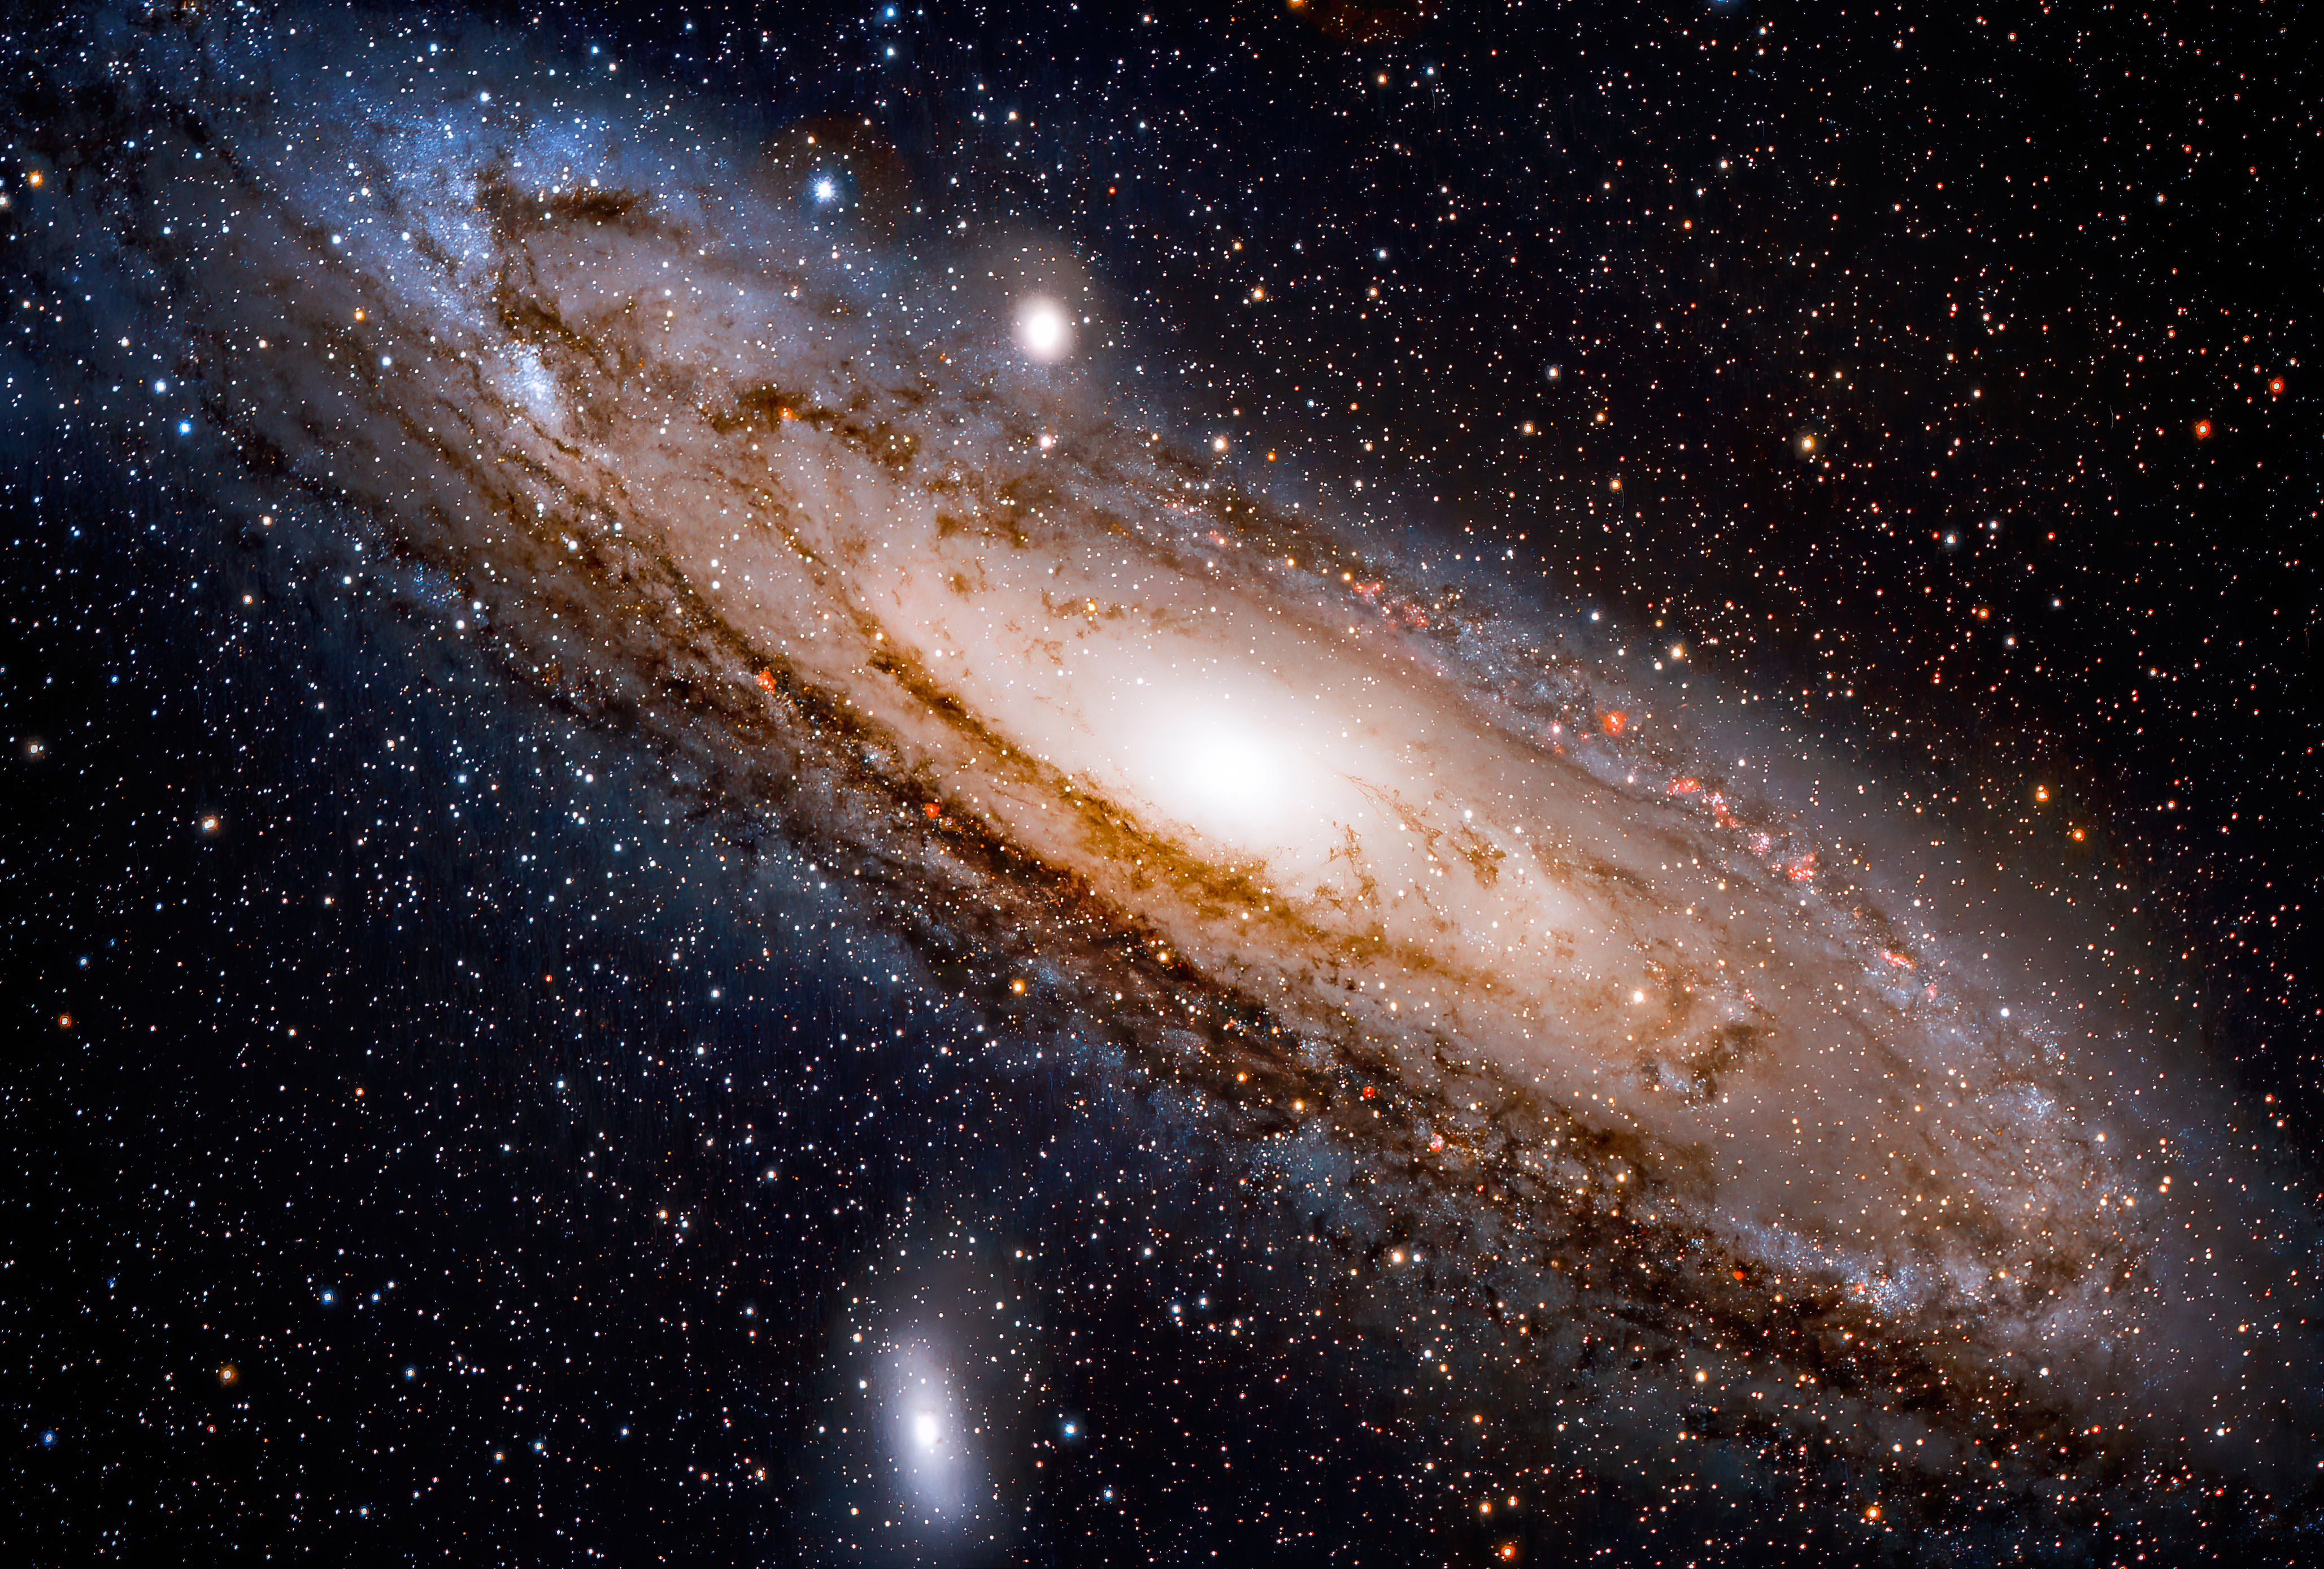
\includegraphics[scale = 0.2]{Andromeda_Galaxy_560mm_FL.jpg}
    \caption{Figure caption describing any symbols and equations on the figure, as well as what is being plotted if it is a plot.\cite{WikipediaAndromeda}}
    \label{fig:figRef}
\end{figure}

Figure captions appear below figures, but Table captions appear above. I have no idea why.


\section{Discussion}

Compare your obtained values to the expected ones using the t-test. Comment on the agreement and possible sources of errors (random and systematic). Make sure that the errors are reasonable given your results.


\section{Conclusion}

Report values again and comment on their agreement with accepted values. Provide any concluding thoughts. For this class, this section should be short.



\clearpage


%\section{References}

\begin{thebibliography}{9}

\bibitem{WikipediaAndromeda}
Wikipedia (2022) "Andromeda Galaxy," \url{https://en.wikipedia.org/wiki/Andromeda_Galaxy#/media/File:Andromeda_Galaxy_560mm_FL.jpg}

\bibitem{uncertaintyManual}
Christopher Cully (2018) "Measurement Uncertainty," University of Calgary, Department of Physics and Astronomy
\end{thebibliography}

%\section{References}
%References appear on their own separate page. To find details about inputting references in \LaTeX{}, refer to \textbf{\href{https://www.overleaf.com/learn/latex/Bibliography_management_with_bibtex}{this page}. }Note that different journals have different referencing styles, and as of late many of created bibtex style packages to convey this. The currently chosen style is the basic ``plain" style, but if you wish you can go to the AIP website and download their personal .bst style file, for example.
%\bibliographystyle{plain}
%\bibliography{Refs}
%\nocite{*}



\end{document}


%%%%%% END %%%%%%%%%%%%%